% Portfólio de Aprendizagem por Projetos Integrados (API) - versão ABNT
% Modelo de referência: "TG Portfólio ABNT - Modelo ADS-BD.pdf" (Fatec São José dos Campos)
% Compilação: latexmk -pdf portfolio-abnt.tex

\documentclass[12pt,a4paper]{article}

% ---------------------------------------------------------------------------
% Idioma, codificação e fonte (Times New Roman, tamanho 12)
% ---------------------------------------------------------------------------
\usepackage[T1]{fontenc}
\usepackage[utf8]{inputenc}
\usepackage[brazilian]{babel}
\usepackage{newtxtext}

% ---------------------------------------------------------------------------
% Página A4: margens superior e esquerda de 3 cm, inferior e direita de 2 cm
% ---------------------------------------------------------------------------
\usepackage[a4paper,top=3cm,left=3cm,bottom=2cm,right=2cm,headheight=15pt,headsep=0.8cm]{geometry}

% Espaçamento de 1,5 linha, texto justificado e recuo de parágrafo de 1,25 cm
\usepackage{setspace}
\onehalfspacing
\usepackage{indentfirst}
\setlength{\parindent}{1.25cm}
\setlength{\parskip}{0pt}

\usepackage{graphicx}
\usepackage{float}
\usepackage{pdfpages}
\usepackage{booktabs}
\usepackage{array}
\usepackage[table]{xcolor}
\usepackage[labelsep=endash,justification=centering,singlelinecheck=false]{caption}
\usepackage{enumitem}
\usepackage{xurl}
\usepackage[hidelinks]{hyperref}
\urlstyle{same}

% ---------------------------------------------------------------------------
% Numeração de páginas no canto superior direito, tamanho 10
% ---------------------------------------------------------------------------
\usepackage{fancyhdr}
\fancypagestyle{plain}{%
  \fancyhf{}%
  \fancyhead[R]{\footnotesize\thepage}%
  \renewcommand{\headrulewidth}{0pt}%
}
\pagestyle{plain}

% ---------------------------------------------------------------------------
% Títulos: capítulos em negrito, tamanho 14, numerados sem o termo "capítulo";
% subitens em negrito, tamanho 12, numerados a partir do capítulo
% ---------------------------------------------------------------------------
\usepackage{titlesec}
\titleformat{\section}{\fontsize{14}{17}\selectfont\bfseries}{\thesection.}{0.4em}{}
\titlespacing*{\section}{0pt}{0pt}{6pt}
\titleformat{\subsection}{\normalsize\bfseries}{\thesubsection}{0.5em}{}
\titlespacing*{\subsection}{0pt}{12pt}{0pt}

% Sumário
\usepackage{tocloft}
\addto\captionsbrazilian{\renewcommand{\contentsname}{SUMÁRIO}}
\renewcommand{\cfttoctitlefont}{\hfill\large\bfseries}
\renewcommand{\cftaftertoctitle}{\hfill}
\renewcommand{\cftsecaftersnum}{.}
\renewcommand{\cftsecleader}{\bfseries\cftdotfill{\cftdotsep}}
\renewcommand{\cftsubsecfont}{\normalfont}
\renewcommand{\cftsubsecpagefont}{\normalfont}
\setlength{\cftsubsecindent}{1.25cm}
\setlength{\cftbeforesecskip}{6pt}

% ---------------------------------------------------------------------------
% Comandos do documento
% ---------------------------------------------------------------------------
% Primeira ocorrência de um termo do glossário em cada seção: itálico com link
\newcommand{\termo}[2]{\hyperlink{gls:#1}{\textit{#2}}}
% Entrada do glossário
\newcommand{\entradaglossario}[3]{\item[\hypertarget{gls:#1}{#2}] #3}
% Título de elemento pré-textual ou pós-textual sem numeração
\newcommand{\titulocentralizado}[1]{\begin{center}\large\textbf{#1}\end{center}\vspace{12pt}}
\newcommand{\titulosemnumero}[1]{%
  \phantomsection\addcontentsline{toc}{section}{#1}%
  {\noindent\fontsize{14}{17}\selectfont\bfseries #1\par}\vspace{6pt}}
% Fonte de tabelas e figuras
\newcommand{\fonte}[1]{\par\vspace{2pt}{\noindent\hspace{0.6cm}Fonte: #1\par}}

% Dados do trabalho
\newcommand{\autor}{PEDRO FELIPE SOUSA GARCIA}
\newcommand{\titulotrabalho}{PORTFÓLIO DE APRENDIZAGEM POR\\PROJETOS INTEGRADOS (API) E\\SYNAPSE: SIMULAÇÃO DE REGRAS DE\\COMISSIONAMENTO COM INTELIGÊNCIA\\ARTIFICIAL}
\newcommand{\natureza}{Trabalho de Graduação apresentado à Faculdade de Tecnologia de São José dos Campos, como parte dos requisitos necessários para a obtenção do título de Tecnólogo em Análise e Desenvolvimento de Sistemas.}
\newcommand{\orientador}{Prof. Me. José Walmir Gonçalves Duque}
\newcommand{\ano}{2026}

\hypersetup{pdftitle={Portfólio de Aprendizagem por Projetos Integrados (API) e Synapse},pdfauthor={Pedro Felipe Sousa Garcia}}

\newcounter{paginasalvas}

\begin{document}

\pagenumbering{roman}

% ===========================================================================
% CAPA
% ===========================================================================
\begin{titlepage}
\thispagestyle{empty}
\begin{center}
\textbf{FACULDADE DE TECNOLOGIA DE SÃO JOSÉ DOS CAMPOS}\\
\textbf{FATEC PROFESSOR JESSEN VIDAL}

\vspace*{\fill}
\textbf{\autor}
\vspace*{\fill}

{\fontsize{14}{18}\selectfont\textbf{\titulotrabalho}}

\vspace*{\fill}
\vspace*{\fill}
São José dos Campos\\
\ano
\end{center}
\end{titlepage}
\setcounter{page}{2}

% ===========================================================================
% FOLHA DE ROSTO
% ===========================================================================
\begin{center}
\textbf{\autor}

\vspace*{\fill}
{\fontsize{14}{18}\selectfont\textbf{\titulotrabalho}}
\vspace*{\fill}
\end{center}

\noindent\hfill\begin{minipage}{8cm}
\singlespacing
\natureza
\end{minipage}

\vspace{2cm}
\noindent\hfill\textbf{Orientador: \orientador}

\vspace*{\fill}
\begin{center}
São José dos Campos\\
\ano
\end{center}
\clearpage

% ===========================================================================
% FOLHA DE APROVAÇÃO
% ===========================================================================
\begin{center}
\textbf{\autor}

\vspace{2cm}
{\fontsize{14}{18}\selectfont\textbf{\titulotrabalho}}
\end{center}

\vspace{1cm}
\noindent\hfill\begin{minipage}{8cm}
\singlespacing
\natureza
\end{minipage}

\vspace{1.5cm}
\begin{center}
\singlespacing
\rule{12cm}{0.4pt}\\
\textbf{Prof. Me. José Walmir Gonçalves Duque -- Fatec-SJC}

\vspace{1.4cm}
\rule{12cm}{0.4pt}\\
\textbf{\textcolor{red}{[TODO: titulação e nome do 1º componente da banca – sigla da instituição]}}

\vspace{1.4cm}
\rule{12cm}{0.4pt}\\
\textbf{\textcolor{red}{[TODO: titulação e nome do 2º componente da banca – sigla da instituição]}}

\vspace{1.4cm}
\rule{1.2cm}{0.4pt}/\rule{1.2cm}{0.4pt}/\rule{1.2cm}{0.4pt}\\
\textbf{DATA DA APROVAÇÃO}
\end{center}
\clearpage

% ===========================================================================
% AGRADECIMENTOS
% ===========================================================================
\titulocentralizado{AGRADECIMENTOS}

\textcolor{red}{[TODO: texto dos agradecimentos, com no máximo uma página]}
\clearpage

% ===========================================================================
% RESUMO
% ===========================================================================
\titulocentralizado{RESUMO}

\noindent Este trabalho apresenta o portfólio dos seis projetos de Aprendizagem por Projetos Integrados (API)
que o autor desenvolveu entre 2024 e 2026 no curso de Tecnologia em Análise e Desenvolvimento de Sistemas da
Fatec São José dos Campos, com destaque para o Synapse, aplicação web que simula o custo de regras de comissionamento
de vendas descritas por texto ou voz. Cada projeto atendeu a uma demanda real de uma empresa parceira e
foi conduzido com o Scrum, de modo que o autor exerceu, ao longo do curso, os papéis de desenvolvedor,
Product Owner e Scrum Master. O documento descreve, para cada projeto, o problema proposto,
a solução desenvolvida pela equipe, o papel do autor e as tecnologias utilizadas, e relaciona essas experiências
a obras de referência das disciplinas do curso. No Synapse, projeto em parceria com a Dom Rock,
o autor atuou como Scrum Master e foi responsável pela arquitetura do sistema. A solução combina um serviço
de inteligência artificial, que converte a descrição da regra em código Python, com a execução desse código
em um container isolado, que recalcula o comissionamento de meses passados e o compara com o comissionamento
pela regra vigente. Como nenhum valor é calculado pelo modelo de linguagem, todos os resultados podem ser conferidos
e auditados. Os projetos evoluíram de uma aplicação web monolítica, no primeiro semestre,
para um sistema de quatro serviços com comunicação por eventos, no sexto semestre. Conclui-se que a aprendizagem
por projetos integrados desenvolveu, além das competências técnicas, a capacidade de registrar decisões,
negociar contratos entre equipes e responder pela operação do sistema depois da entrega.

\vspace{12pt}
\noindent\textbf{Palavras-Chave:} Aprendizagem por Projetos Integrados; Arquitetura orientada a eventos; Inteligência artificial generativa; Scrum; Simulação de comissionamento.
\clearpage

% ===========================================================================
% ABSTRACT
% ===========================================================================
\titulocentralizado{ABSTRACT}

\noindent This work presents the portfolio of the six Integrated Project-Based Learning (API) projects that the author developed between 2024 and 2026 in the Systems Analysis and Development technology program at Fatec São José dos Campos, highlighting Synapse, a web application that simulates the cost of sales commission rules described by text or voice. Each project addressed a real demand from a partner company and was conducted with Scrum, so that the author performed, throughout the program, the roles of developer, Product Owner and Scrum Master. For each project, the document describes the proposed problem, the solution developed by the team, the author's role and the technologies used, and relates these experiences to reference works from the program's courses. In Synapse, a project in partnership with Dom Rock, the author acted as Scrum Master and was responsible for the system architecture. The solution combines an artificial intelligence service, which converts the rule description into Python code, with the execution of that code in an isolated container, which recalculates the commissions of past months and compares them with the commissions under the current rule. Because no value is calculated by the language model, every result can be checked and audited. The projects evolved from a monolithic web application, in the first semester, to a system of four services communicating through events, in the sixth semester. The work concludes that integrated project-based learning developed, in addition to technical skills, the ability to record decisions, negotiate contracts between teams and take responsibility for operating the system after delivery.

\vspace{12pt}
\noindent\textbf{Keywords:} Integrated Project-Based Learning; Event-driven architecture; Generative artificial intelligence; Scrum; Commission simulation.
\clearpage

% ===========================================================================
% SUMÁRIO
% ===========================================================================
\tableofcontents
\clearpage

% ===========================================================================
% ELEMENTOS TEXTUAIS: numeração arábica que continua a contagem das folhas
% ===========================================================================
\setcounter{paginasalvas}{\value{page}}
\pagenumbering{arabic}
\setcounter{page}{\value{paginasalvas}}

% ===========================================================================
\section{INTRODUÇÃO}
% ===========================================================================

O Synapse é o projeto de API do sexto semestre, desenvolvido entre 26/08/2026 e 22/11/2026 em parceria com a Dom Rock, empresa de inteligência de dados e inteligência artificial (TITUS SYSTEMS, 2026a). Esta introdução apresenta o projeto em detalhe, porque ele dá título a este trabalho e reúne as competências desenvolvidas ao longo do curso. As subseções a seguir descrevem o problema proposto, a relevância desse problema, a solução e a arquitetura do sistema, os mecanismos de validação e auditoria, as tecnologias, o papel do autor e os resultados obtidos.

% ---------------------------------------------------------------------------
\subsection{Contexto e problema}
% ---------------------------------------------------------------------------

As empresas do varejo alteram com frequência as regras de comissionamento de vendas. A cada mês, entram em vigor percentuais que valem apenas naquele mês, bônus por faixa de valor vendido, acréscimos sazonais, como os da Black Friday, e exceções para determinados cargos. Essas regras chegam em texto livre e não ficam registradas de forma estruturada, o que causa perda de conhecimento, conflitos entre regras e falta de rastreabilidade. Além disso, a empresa não sabe, antes de aplicar uma regra nova, quanto ela custaria e se caberia no orçamento, nem consegue explicar depois a um auditor a origem de cada valor pago.

Para caracterizar o problema, a Dom Rock forneceu os dados de seis \termo{competencia}{competências} (meses de referência da apuração) de uma rede varejista, de julho a dezembro de 2025, e uma especificação das regras de comissionamento. Os dados estão divididos em três bases relacionadas por competência. A base de recursos humanos traz funcionário, cargo, loja, marca e datas de admissão e demissão, com 469 funcionários em novembro de 2025. A base de vendas traz os lançamentos de venda por funcionário, com 5.000 linhas e R\$~13,85 milhões vendidos no mesmo mês. Por fim, a base de comissionamento traz o percentual de cada uma das 30 combinações de marca e cargo.

A análise da especificação mostrou que ela tem três camadas, e cada camada exige um tratamento diferente no sistema. A primeira camada reúne as regras base, que valem em todas as competências, como a aplicação do percentual por marca e cargo, o cálculo do gerente sobre a venda total da loja e a proporcionalidade por dias trabalhados em admissões, demissões, afastamentos e férias. A segunda camada reúne os eventos de recursos humanos, como atestados, férias e licenças, que só existem em texto e não aparecem em nenhuma coluna das bases. Já a terceira camada reúne as regras de cada competência, como um percentual maior apenas em novembro ou um bônus para vendas acima de R\$~40 mil, e são essas regras que mudam de forma a cada mês. Como consequência, o sistema precisava expressar uma lógica que varia de estrutura, e não apenas de valores, o que uma fórmula fixa não consegue fazer.

% ---------------------------------------------------------------------------
\subsection{Relevância}
% ---------------------------------------------------------------------------

O problema é relevante porque a remuneração variável afeta diretamente o custo da operação e a confiança dos vendedores na empresa. Uma regra mal calculada gera prejuízo financeiro e, ao mesmo tempo, questionamentos trabalhistas. Além disso, uma regra pode caber no orçamento em um mês de vendas fracas e ultrapassá-lo em um mês de pico, de modo que a pergunta útil para a empresa não é se a regra cabe em um mês, e sim se ela se sustenta ao longo do tempo.

A automação desse cálculo com inteligência artificial generativa, porém, traz um risco próprio, porque \termo{modelo}{modelos de linguagem} que geram código produzem com frequência programas que executam sem erro, mas não resolvem corretamente o problema proposto (CHEN \textit{et al.}, 2021). No caso das comissões, esse tipo de erro produz um valor plausível e errado, que ninguém percebe sem conferir o cálculo. Por isso, a solução precisava usar a inteligência artificial para interpretar a linguagem natural sem permitir que ela determinasse os valores pagos, e precisava registrar cada etapa para que um auditor pudesse reconstruir a origem de qualquer resultado.

% ---------------------------------------------------------------------------
\subsection{Solução e arquitetura}
% ---------------------------------------------------------------------------

A equipe desenvolveu uma aplicação web em que o profissional de recursos humanos descreve a regra de comissionamento por texto ou por voz, informa o orçamento disponível e escolhe as competências que deseja simular. O sistema recalcula o comissionamento dessas competências como se a regra nova estivesse em vigor e compara o resultado com o comissionamento calculado pela regra vigente, chamado de \termo{baseline}{baseline}. Essa técnica, chamada de \termo{backtesting}{backtesting}, mantém as mesmas vendas, os mesmos funcionários e os mesmos eventos de recursos humanos e muda apenas a regra. Assim, qualquer diferença entre o valor simulado e o baseline é causada pela regra, e não por uma previsão de vendas que poderia estar errada.

O sistema tem quatro serviços, mostrados na Figura~\ref{fig:arquitetura}. O frontend é a interface usada pelo profissional de recursos humanos e pelo auditor. A API recebe as requisições, controla o estado de cada simulação e envia o progresso ao frontend por eventos enviados pelo servidor (SSE). O serviço de inteligência artificial (\texttt{codegen}) interpreta a regra e gera o código que a implementa. Por fim, o serviço de execução (\texttt{worker}) é o único autorizado a executar esse código.

\begin{figure}[tbp]
\centering
\caption{Arquitetura do Synapse}
\label{fig:arquitetura}
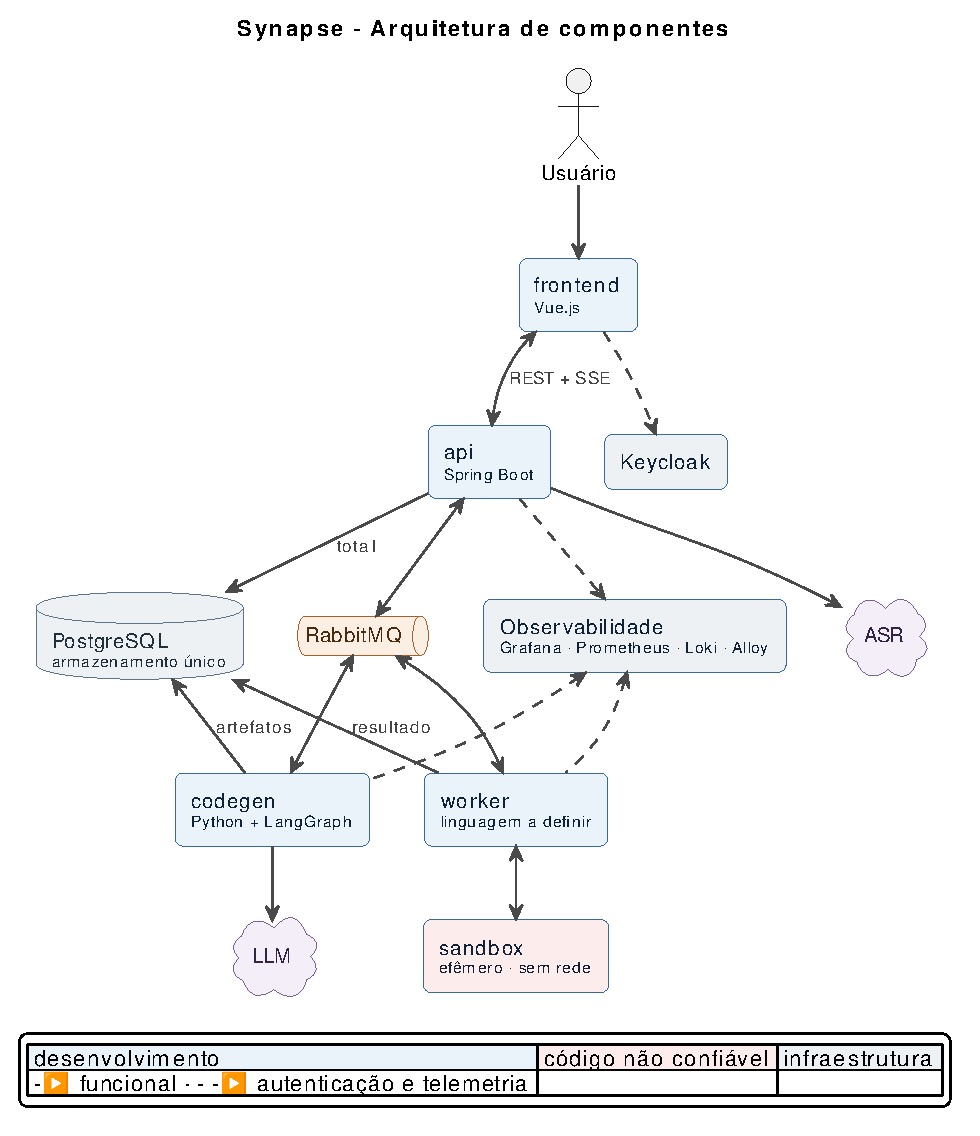
\includegraphics[width=0.62\textwidth]{figuras/arquitetura_synapse.pdf}
\fonte{TITUS SYSTEMS (2026a).}
\end{figure}

Uma simulação percorre os serviços na seguinte ordem. Primeiro, a API grava a descrição da regra e, quando ela chega por voz, transcreve o áudio. Em seguida, o serviço de inteligência artificial extrai da descrição uma representação estruturada da regra, com um núcleo (vigência, loja, marca, cargo e percentual) e os demais elementos que o usuário especificou, como faixas de valor, janelas de datas e exclusões. Uma validação determinística confere essa representação antes da geração do código. Quando encontra um problema, como uma competência fora das disponíveis ou um orçamento negativo, o sistema abre um chat de correção, em que o usuário corrige a regra por texto ou por voz; quando não encontra, o fluxo segue sem pedir confirmação. Depois, o serviço de inteligência artificial gera o código Python da regra e o serviço de execução o executa sobre os dados das competências escolhidas. Por fim, o serviço de execução compara o resultado com o baseline, aplica o critério de orçamento e grava o resultado da simulação.

Quando a regra ultrapassa o orçamento, o sistema propõe uma alternativa. Em até três tentativas, o serviço de inteligência artificial reduz na mesma proporção todos os percentuais da regra, preserva os demais elementos e simula cada versão antes de apresentá-la. Quando a regra cabe no orçamento, o sistema calcula a maior meta de vendas que o orçamento suporta, simulando o mesmo código em metas diferentes. Em nenhum dos dois casos o modelo de linguagem estima valores, porque todo percentual, meta e comissão apresentado ao usuário vem de uma execução real do código.

A comunicação entre os serviços segue três regras, registradas na documentação de arquitetura do projeto. A primeira é que os serviços internos nunca se chamam diretamente e trocam mensagens apenas pelo RabbitMQ, em uma \termo{eventos}{arquitetura orientada a eventos}. Como as etapas de inteligência artificial e de execução levam de segundos a minutos, uma chamada síncrona bloquearia o usuário e acoplaria os serviços ao ritmo do mais lento (NEWMAN, 2021). A segunda regra é que cada mensagem carrega apenas a referência de um registro do banco, e não o conteúdo, de modo que áudios, códigos e resultados ficam no PostgreSQL e o broker de mensagens permanece leve. A terceira regra é que a API grava cada alteração de estado e a mensagem correspondente na mesma transação do banco, segundo o padrão \termo{outbox}{outbox transacional} (RICHARDSON, 2018), o que impede que uma simulação mude de estado sem que os demais serviços sejam avisados. Além disso, cada serviço acessa o banco com um usuário próprio, cujas permissões se restringem às tabelas que o serviço precisa ler ou escrever. Por isso, o serviço de inteligência artificial não consegue alterar o estado de uma simulação nem a trilha de auditoria, mesmo que seu código tenha um erro.

O código gerado é tratado como não confiável, porque pode conter erros do modelo ou instruções maliciosas inseridas no texto da regra. Por isso, o serviço de execução roda cada código em um \termo{container}{container} Docker criado apenas para aquela execução, sem acesso à rede, com usuário sem privilégios de administrador, sistema de arquivos somente leitura, limites de processamento e memória e tempo máximo de execução. Como o container não tem rede, os dados das cinco competências usadas e os baselines já vêm incluídos na imagem Docker. Além disso, o critério de orçamento é aplicado fora do container, de modo que o código gerado não consegue alterar o veredito sobre a viabilidade da regra.

% ---------------------------------------------------------------------------
\subsection{Validação, auditoria e explicação dos resultados}
% ---------------------------------------------------------------------------

O princípio central do Synapse é que nenhum valor sai do \termo{modelo}{modelo de linguagem}. O modelo interpreta o texto da regra, escreve o código e redige a explicação do resultado, mas toda conta é feita por código determinístico executado sobre os dados reais. Esse princípio sustenta a auditoria, porque cada valor pode ser recalculado a partir do código armazenado e dos dados, sem depender de uma nova geração pelo modelo.

O isolamento do \termo{container}{container} garante que o código gerado não seja perigoso, mas não garante que ele esteja correto. Por isso, o sistema aplica verificações determinísticas em toda simulação. Dentro do container, asserções conferem que nenhuma comissão é negativa, que toda comissão positiva tem uma origem rastreável, como uma venda, um evento de recursos humanos remunerado ou um bônus da competência, e que a soma das comissões por loja é igual à soma por funcionário. Fora do container, o serviço de execução confere que cada elemento declarado na regra foi de fato aplicado antes de emitir o resultado. Quando uma dessas verificações falha, o sistema interrompe a simulação e informa o motivo ao usuário, em vez de apresentar um valor incompleto.

Para a auditoria, cada etapa do serviço de inteligência artificial grava seus artefatos no banco, como o \textit{prompt} enviado, a resposta do modelo e o código gerado, e publica uma mensagem com a referência desses artefatos. A API registra essas mensagens em uma trilha associada à simulação, com identificador, data e hora, versão da regra aplicada e fontes de dados usadas. O auditor não participa do fluxo de simulação e consulta essa trilha em uma área própria do sistema, que reúne a conversa com o usuário, o código Python, as fontes de dados, o modelo de transcrição usado e o áudio das entradas por voz.

A explicação do resultado ao usuário segue o mesmo princípio. O modelo de linguagem redige um texto que narra os valores apurados, e o sistema confere, por código, que todo número citado nesse texto existe no resultado da simulação, inclusive os números escritos por extenso. Quando a explicação falha nessa conferência, o sistema não a exibe, mantém o resultado e marca a simulação com um alerta de baixa rastreabilidade, porque uma falha de explicação reduz a rastreabilidade, mas não invalida o valor calculado.

Por fim, a equipe decidiu não usar \termo{rag}{RAG}, técnica que recupera trechos de uma base de conhecimento e os inclui no contexto do modelo (LEWIS \textit{et al.}, 2020). Como o esquema das bases, as regras base e a especificação completa cabem no \textit{prompt}, uma busca por trechos tornaria o contexto incompleto sem resolver nenhum problema do projeto. A decisão registra que essa técnica passa a fazer sentido quando o volume de regras históricas crescer a ponto de exigir a detecção de conflitos entre elas.

% ---------------------------------------------------------------------------
\subsection{Tecnologias}
% ---------------------------------------------------------------------------

A escolha das tecnologias partiu de dois conjuntos de restrições. A Fatec e a Dom Rock exigiram Vue.js no frontend, Spring Boot na API, um modelo de linguagem acessado por API pública, um framework da família LangChain e o uso obrigatório de inteligência artificial generativa no desenvolvimento. As demais tecnologias foram escolhidas pela função de cada serviço, conforme a Tabela~\ref{tab:tecnologias}.

\begin{table}[tbp]
\centering
\caption{Tecnologias do Synapse}
\label{tab:tecnologias}
\renewcommand{\arraystretch}{1.1}
\begin{tabular}{p{4.6cm} p{10.4cm}}
\toprule
\textbf{Tecnologia} & \textbf{Função no sistema} \\
\midrule
Vue.js, Pinia e Tailwind CSS & Interface de entrada da regra, chat de correção, resultados, histórico e área do auditor \\
Java e Spring Boot & API, controle do estado das simulações e envio do progresso por SSE \\
Python e LangGraph & Serviço de inteligência artificial, organizado como um grafo de etapas (LANGCHAIN, 2026) \\
Gemini & Modelo de linguagem usado na extração da regra, na geração do código e na explicação \\
Deepgram & Transcrição dos áudios, escolhida após a avaliação de 27 áudios reais pela equipe \\
Python e Docker & Serviço de execução e container isolado em que o código gerado roda \\
RabbitMQ & Único canal de comunicação entre a API e os serviços de inteligência artificial e de execução \\
PostgreSQL & Banco único do sistema, com um usuário de acesso por serviço \\
Keycloak & Autenticação dos usuários com OIDC e emissão dos tokens validados pela API \\
JSON Schema & Contratos das mensagens e das rotas, validados na integração contínua \\
Grafana, Prometheus e Loki & Logs e métricas correlacionados pelo identificador de cada simulação \\
GitHub Actions & Verificação de cada serviço e deploy independente no ambiente de homologação \\
\bottomrule
\end{tabular}
\fonte{Elaborado por GARCIA, (\ano).}
\end{table}

% ---------------------------------------------------------------------------
\subsection{Papel do autor}
% ---------------------------------------------------------------------------

No Synapse, o autor atuou como \termo{sm}{Scrum Master} e foi responsável pela arquitetura do sistema, além de ter sido o integrante com mais commits no repositório (183 de 402). Como Scrum Master, definiu o fluxo de trabalho da equipe, em que cada funcionalidade é desenvolvida em uma branch própria, revisada por pelo menos um colega e validada pela \termo{po}{Product Owner} no ambiente de homologação antes de chegar à versão principal. Também organizou as tarefas no GitHub Projects, com uma automação que move para a coluna de tarefas prontas aquelas cujas dependências foram resolvidas, e resolveu impedimentos de escopo ao longo das \termo{sprint}{sprints}, com as decisões registradas na documentação do projeto. Essas atividades correspondem às responsabilidades do Scrum Master descritas por Schwaber e Sutherland (2020). \textcolor{red}{[TODO: como o autor conduziu as cerimônias Scrum no Synapse (daily, planning, review e retrospectiva), com frequência, formato e um exemplo concreto]}

Como o uso de inteligência artificial generativa no desenvolvimento era obrigatório, o autor também definiu como a equipe deveria usá-la. Cada serviço recebeu instruções próprias para os assistentes de código, com as regras de segurança daquele serviço, e um script de verificação com compilação, tipagem, análise estática e testes. Um gancho executado antes de cada commit roda a verificação apenas dos serviços alterados, e a integração contínua roda o mesmo comando, de modo que o código gerado com apoio de inteligência artificial passa pelos mesmos critérios que o código escrito manualmente.

Como responsável pela arquitetura, o autor registrou as decisões em documentos versionados, chamados de ADRs (\textit{Architecture Decision Records}), com o contexto, a decisão e as consequências de cada uma. Esses registros cobrem a arquitetura orientada a eventos, a organização dos quatro serviços em um único repositório, a coleta centralizada de logs e métricas e o fluxo de trabalho com inteligência artificial. Além disso, o autor modelou o domínio a partir dos dados da Dom Rock, definiu a simulação como recálculo de competências passadas e escreveu os \termo{contrato}{contratos de dados} em JSON Schema, que permitiram aos quatro serviços avançar em paralelo.

Na implementação, o autor contribuiu com todos os serviços. Na API, implementou o outbox transacional, o consumo dos eventos de progresso e de simulação concluída, o envio do progresso ao frontend e a integração com o Keycloak e com a transcrição. No serviço de inteligência artificial, implementou a extração do orçamento, da meta e do período a partir do texto, a sugestão de regra alternativa, a validação das janelas de datas e a conferência dos números citados na explicação. No serviço de execução, criou a imagem do container, a verificação de que cada elemento da regra foi aplicado e o registro das fontes de dados de cada execução. Por fim, no frontend, implementou o chat de correção e partes da área do auditor.

% ---------------------------------------------------------------------------
\subsection{Resultados}
% ---------------------------------------------------------------------------

A equipe organizou o desenvolvimento em três \termo{sprint}{sprints}, com as entregas resumidas na Tabela~\ref{tab:sprints}. Cada sprint terminou com a validação das \textit{user stories} pela Product Owner, do ponto de vista do cliente, e com um vídeo de demonstração dos incrementos.

\begin{table}[H]
\centering
\caption{Entregas das sprints do Synapse}
\label{tab:sprints}
\renewcommand{\arraystretch}{1.1}
\begin{tabular}{p{1.3cm} p{2.2cm} p{11.2cm}}
\toprule
\textbf{Sprint} & \textbf{Entrega} & \textbf{Funcionalidades entregues} \\
\midrule
1 & 27/09/2026 & Entrada da regra por formulário, geração do código, execução isolada, comparação com o baseline, alerta de inviabilidade e histórico das regras \\
2 & 25/10/2026 & Entrada da regra por texto livre e por voz, chat de correção, sugestão automática de ajuste e cálculo da meta de vendas que cabe no orçamento \\
3 & 22/11/2026 & Trilha de auditoria, área do auditor, explicação do resultado com conferência numérica e alerta de baixa rastreabilidade \\
\bottomrule
\end{tabular}
\fonte{Elaborado por GARCIA, (\ano).}
\end{table}

Com essas entregas, o sistema simula uma regra de comissionamento descrita em linguagem natural sobre as cinco competências publicadas (agosto a dezembro de 2025), compara o custo com o baseline e com o orçamento e registra cada etapa para auditoria. A apresentação final está marcada para a Feira de Soluções de 03/12/2026.

O sistema tem duas limitações, declaradas ao usuário e acordadas com o cliente. A primeira é que o backtesting mantém o comportamento histórico das vendas e, portanto, não estima como uma comissão diferente alteraria o volume vendido. A segunda é que o baseline é calculado pelo próprio sistema a partir das regras da especificação, e não pelo valor que a empresa efetivamente pagou, que não faz parte dos dados fornecidos. Por isso, as diferenças apresentadas medem o efeito da regra dentro do modelo de cálculo implementado, e a validação contra os valores reais depende de dados que só a Dom Rock pode fornecer.

% ---------------------------------------------------------------------------
\subsection{Organização do documento}
% ---------------------------------------------------------------------------

Além desta introdução, o documento tem mais dois capítulos. O Capítulo~2 descreve os seis projetos de API em ordem cronológica. O Capítulo~3 apresenta as considerações finais sobre a trajetória do autor no curso. Por fim, o Apêndice~A reúne o portfólio completo.

% ===========================================================================
\clearpage
\section{PROJETOS}
% ===========================================================================

Os projetos de API correspondem às atividades desenvolvidas ao longo da graduação, organizadas cronologicamente por ano e semestre. Cada projeto integrador partiu de uma demanda real proposta por docentes ou empresas parceiras, com o objetivo de aplicar na prática os conhecimentos adquiridos no curso. Em todos os projetos, a equipe trabalhou com o Scrum, em \termo{sprint}{sprints} de duração fixa, revisadas com o cliente ao final de cada ciclo. As subseções a seguir apresentam uma síntese de cada projeto, e o portfólio completo pode ser consultado no Apêndice~A. A Tabela~\ref{tab:projetos} lista os projetos e os respectivos repositórios no GitHub.

\begin{table}[H]
\centering
\caption{Lista de Projetos API}
\label{tab:projetos}
\renewcommand{\arraystretch}{1.1}
\begin{tabular}{p{6.4cm} p{8.6cm}}
\toprule
\textbf{Título do Projeto} & \textbf{Link do GitHub} \\
\midrule
Mestre Ágil (1º semestre) & \url{https://github.com/Titus-System/1Semestre-ADS} \\
IdScan (2º semestre) & \url{https://github.com/Titus-System/2semestre-ADS} \\
InsightFlow (3º semestre) & \url{https://github.com/Titus-System/3Semestre-ADS-Backend} \\
NEXA (4º semestre) & \url{https://github.com/Titus-System/Nexa-api} \\
SyncDesk (5º semestre) & \url{https://github.com/Titus-System/SyncDesk} \\
Synapse (6º semestre) & \url{https://github.com/Titus-System/synapse} \\
\bottomrule
\end{tabular}
\fonte{Elaborado por GARCIA, (\ano).}
\end{table}

% ---------------------------------------------------------------------------
\subsection{ANO 1 – 1º semestre: Mestre Ágil}
% ---------------------------------------------------------------------------

O Mestre Ágil foi desenvolvido no primeiro semestre de 2024 (TITUS SYSTEMS, 2024b). A empresa parceira foi a própria Fatec São José dos Campos, por meio do CADI (Centro de Aprendizagem em Desenvolvimento e Integração), o Departamento de Extensão, com o Professor Antônio Egydio no papel de cliente. O problema proposto era que estudantes e profissionais que começam a adotar o Scrum aprendem o método em conteúdos fragmentados, sem padronização e sem avaliações que confirmem o aprendizado. Por isso, essas equipes demoram a amadurecer e aplicam de forma incorreta os papéis, os eventos e os artefatos definidos no Guia do Scrum (SCHWABER; SUTHERLAND, 2020). A contribuição pretendida era facilitar a compreensão do Scrum por meio de uma abordagem prática e com avaliação do aprendizado.

O autor atuou como desenvolvedor. A equipe construiu uma plataforma web responsiva que reúne conteúdo teórico, exemplos práticos, ferramentas de apoio, como o \termo{backlog}{backlog} e o gráfico de burndown, e um sistema de avaliações com emissão de certificado. Na plataforma, o usuário estuda o conteúdo, responde aos questionários e, quando aprovado na prova final, recebe um certificado em PDF, enquanto o administrador consulta o desempenho dos usuários.

No desenvolvimento, o autor implementou as rotas de autenticação com a biblioteca Flask-Login, as rotas de perfil do usuário, o processamento do resultado dos questionários e da prova final e a emissão do certificado. Além disso, definiu o uso de arquivos JSON para armazenar o conteúdo teórico, as perguntas e a justificativa de cada erro. Esse formato funcionou como \termo{contrato}{contrato de dados} e permitiu que frontend, backend e produção de conteúdo avançassem em paralelo. O autor também configurou o \termo{deploy}{deploy} em uma instância AWS EC2, com NGINX como proxy reverso e tráfego HTTPS.

O backend foi escrito em Python com o framework Flask, cuja organização em rotas e templates segue o modelo descrito por Grinberg (2018), e os dados foram armazenados em SQLite. O frontend usou HTML, CSS, Bootstrap e JavaScript, e a equipe usou Git e GitHub para o versionamento e Figma e Krita para os protótipos e as imagens.

% ---------------------------------------------------------------------------
\subsection{ANO 1 – 2º semestre: IdScan}
% ---------------------------------------------------------------------------

O IdScan foi desenvolvido no segundo semestre de 2024 (TITUS SYSTEMS, 2024a). A empresa parceira foi a Fatec São José dos Campos, por meio do CADI, com o Professor Giuliano Bertoti no papel de cliente. O problema proposto era que empresas e instituições que digitalizam documentos de identidade (RG) ainda digitam os dados manualmente, em um processo lento e sujeito a erros. As alternativas baseadas em serviços externos de \termo{ocr}{OCR} e inteligência artificial, porém, têm custo recorrente e esbarram em restrições de privacidade, porque o RG contém dados pessoais sensíveis. A contribuição pretendida era automatizar a extração dos dados sem que eles deixassem o computador do usuário.

O autor atuou como \termo{po}{Product Owner}. Nessa função, conduziu o kick-off com o cliente, levantou os requisitos e elaborou o \termo{backlog}{backlog} do produto. No kick-off, o autor identificou que a exigência de não usar serviços externos era, na verdade, um requisito não funcional de privacidade, e esse requisito passou a orientar todas as decisões técnicas do projeto, conforme a distinção entre requisitos funcionais e não funcionais apresentada por Sommerville (2011). Além disso, o autor organizou o backlog em fatias verticais de valor, de modo que a primeira \termo{sprint}{sprint} já entregou o fluxo completo de extração, ainda executado pelo terminal. Com essa estratégia, a equipe validou com o cliente, na primeira revisão, a viabilidade de executar o OCR e os modelos de linguagem localmente.

A equipe desenvolveu um aplicativo desktop em Java que digitaliza RGs e armazena os dados em um banco MySQL local. No aplicativo, o usuário carrega a imagem do documento, confere os campos preenchidos automaticamente, corrige o que o reconhecimento não captou e salva o registro, que depois pode ser buscado e editado. O reconhecimento de texto usa o Tesseract, cuja arquitetura é descrita por Smith (2007), e os campos são interpretados por \termo{modelo}{modelos de linguagem} executados pelo Ollama.

Como desenvolvedor, o autor implementou a estrutura do aplicativo, o tratamento da imagem antes do reconhecimento, a comunicação com o servidor Ollama e os \textit{prompts} que identificam cada campo do RG. As tecnologias utilizadas foram Java 17, Maven, JavaFX, Tesseract, Ollama, MySQL, Jira, Figma, Git e GitHub.

% ---------------------------------------------------------------------------
\subsection{ANO 2 – 1º semestre: InsightFlow}
% ---------------------------------------------------------------------------

O InsightFlow foi desenvolvido no primeiro semestre de 2025 (TITUS SYSTEMS, 2025a). A empresa parceira foi a Fatec São José dos Campos, por meio do CADI, com o Professor Marcos Nascimento, coordenador do curso de Logística, no papel de cliente. O problema proposto era que profissionais de logística e de comércio exterior que analisam o desempenho do Brasil no comércio internacional dependem de planilhas brutas publicadas pelo Ministério do Desenvolvimento, Indústria, Comércio e Serviços. Como os dados de 2014 a 2024 somam dezenas de milhões de registros em arquivos separados, a consolidação manual é demorada e impede a identificação rápida de tendências. A contribuição pretendida era reunir esses dados em uma ferramenta de análise e previsão.

O autor atuou como desenvolvedor, com foco no backend. A equipe construiu uma plataforma web com painéis interativos, busca por código NCM, comparação entre estados, análises estatísticas e previsão de tendências para 24 meses. Na plataforma, o usuário escolhe o período, os estados ou os produtos de interesse e visualiza os indicadores em gráficos.

O autor implementou o pipeline de limpeza dos dados com Python, Jupyter Notebook e Pandas, configurou a estrutura do servidor Flask adotada pelos demais desenvolvedores e implementou as análises estatísticas. A previsão de tendências usou o modelo SARIMA, que trata séries temporais com sazonalidade (HYNDMAN; ATHANASOPOULOS, 2021). Além disso, na segunda \termo{sprint}{sprint}, o autor identificou que as agregações ultrapassavam o limite de 1 segundo de tempo de resposta. Para resolver essa lentidão, criou índices e visões materializadas no PostgreSQL, recursos descritos por Elmasri e Navathe (2011), e acrescentou um cache em Redis para os ranqueamentos mais pesados. Com essas medidas, todas as rotas passaram a cumprir o requisito de tempo de resposta. O autor também configurou a aplicação em \termo{container}{containers} Docker para o \termo{deploy}{deploy} na AWS.

As tecnologias utilizadas foram Python, Flask, Pandas, NumPy, Scikit-learn, StatsModels, PostgreSQL, Redis, Docker e AWS no backend, e React, TypeScript, Vite e Tailwind CSS no frontend, além de Jira, Figma, Git e GitHub.

% ---------------------------------------------------------------------------
\subsection{ANO 2 – 2º semestre: NEXA}
% ---------------------------------------------------------------------------

O NEXA foi desenvolvido no segundo semestre de 2025 (TITUS SYSTEMS, 2025b). A empresa parceira foi a TecSys Brasil, que atua em comércio exterior e soluções fiscais. O problema proposto era que os analistas fiscais que preparam o registro de importações precisam descrever cada item declarado à Receita Federal, relacionando o código do fabricante (\textit{part-number}), a classificação fiscal (NCM), o fabricante e a origem. Como esse processo é manual e depende de várias fontes, uma descrição incorreta leva a questionamentos, multas e atrasos no desembaraço aduaneiro. A contribuição pretendida era gerar essas descrições automaticamente com agentes de inteligência artificial.

O autor atuou como \termo{po}{Product Owner} e também foi o principal responsável pela API orquestradora. Como Product Owner, levantou os requisitos com a TecSys, escreveu sete \textit{user stories} distribuídas em três \termo{sprint}{sprints}, com critérios de aceitação detalhados, e refinou o \termo{backlog}{backlog} de acordo com o retorno do cliente. Além disso, validou as entregas de cada sprint e gravou os vídeos de demonstração.

A equipe construiu uma aplicação web que recebe um \textit{part-number}, digitado ou extraído de pedidos de compra em PDF, e gera a descrição técnica, a NCM e a alíquota do item. No sistema, o usuário envia o pedido, recebe imediatamente a confirmação de que ele está em processamento e acompanha o progresso em tempo real. Os agentes de inteligência artificial pesquisam o item na internet e usam \termo{rag}{RAG}, técnica que inclui no contexto do \termo{modelo}{modelo de linguagem} trechos recuperados de uma base de conhecimento (LEWIS \textit{et al.}, 2020).

Como desenvolvedor, o autor percebeu que a comunicação inicialmente planejada entre a API e os agentes não suportaria a latência das pesquisas. Por isso, definiu uma \termo{eventos}{arquitetura orientada a eventos} com Redis Pub/Sub entre os dois serviços, enquanto o \termo{websocket}{WebSocket} ficou restrito à comunicação com o frontend, e implementou uma fila de tarefas com Celery. Essas escolhas seguem o princípio de desacoplar produtores e consumidores por meio de mensagens assíncronas (KLEPPMANN, 2017). As tecnologias utilizadas foram Python, Flask, Flask-SocketIO, Celery, Redis, SQLAlchemy, Pydantic, PostgreSQL, Ollama, smol-agents, ChromaDB, PDFPlumber, React, TypeScript, Docker, Pytest, Jira e GitHub.

% ---------------------------------------------------------------------------
\subsection{ANO 3 – 1º semestre: SyncDesk}
% ---------------------------------------------------------------------------

O SyncDesk foi desenvolvido entre 03/03/2026 e 25/06/2026 (TITUS SYSTEMS, 2026b). A empresa parceira foi a Pro4Tech, empresa de software que presta suporte aos produtos que fornece aos seus clientes. O problema proposto era que as demandas dos clientes chegavam ao suporte sem nenhuma classificação, de modo que o atendente precisava descobrir sozinho o produto envolvido e o tipo de demanda. Além disso, o histórico das conversas não ficava registrado em um único lugar, e a gestão não conseguia acompanhar prazos, volume de demandas e desempenho dos atendentes. A contribuição pretendida era estruturar todo o ciclo de atendimento, da triagem ao encerramento.

O autor atuou como desenvolvedor e foi o principal responsável pelo backend, com 117 dos 167 commits do repositório da API. A equipe construiu um aplicativo mobile para os clientes da Pro4Tech, chamados de solicitantes no sistema, e uma aplicação web para atendentes e administradores. No aplicativo, o solicitante passa por um chatbot de triagem que identifica o produto e o tipo de demanda e abre o chamado automaticamente. A partir desse momento, solicitante e atendente conversam em tempo real por \termo{websocket}{WebSocket} até o encerramento e a avaliação do chamado.

No backend, o autor criou a estrutura da API em FastAPI e implementou a autenticação, o chat em tempo real, boa parte do domínio de chamados e os indicadores do painel de gestão. Para que um domínio da API reagisse a ações de outro sem depender diretamente dele, o autor criou um barramento de eventos interno. Além disso, implementou o padrão \termo{outbox}{outbox transacional} para o envio de e-mails, que grava cada mensagem no banco antes do envio e evita perdê-la em caso de falha (RICHARDSON, 2018). O autor também montou o monitoramento com Prometheus, Grafana e Loki, seguindo a prática de acompanhar latência, tráfego, erros e saturação dos serviços (BEYER \textit{et al.}, 2016), e criou o pipeline de \termo{deploy}{deploy} automático em GitHub Actions.

As tecnologias utilizadas foram Python, FastAPI, SQLAlchemy, Alembic, PostgreSQL, MongoDB, JWT, MinIO, Resend, Prometheus, Grafana, Loki, Docker, GitHub Actions e Pytest no backend, React Native e Expo no aplicativo mobile e React, Vite e Tailwind CSS na aplicação web.

% ---------------------------------------------------------------------------
\subsection{ANO 3 – 2º semestre: Synapse}
% ---------------------------------------------------------------------------

O Synapse foi desenvolvido entre 26/08/2026 e 22/11/2026 (TITUS SYSTEMS, 2026a). A empresa parceira foi a Dom Rock, que atua com inteligência de dados e inteligência artificial. O problema proposto era que as regras de comissionamento de vendas mudam com frequência, chegam em texto livre e não ficam registradas de forma estruturada, de modo que a empresa não sabe quanto uma regra nova custaria antes de aplicá-la, nem consegue explicar a um auditor a origem de cada valor pago. A contribuição pretendida era simular o custo de cada regra antes da aplicação e registrar cada etapa dessa simulação.

O autor atuou como \termo{sm}{Scrum Master} e foi responsável pela arquitetura do sistema. A equipe está desenvolvendo uma aplicação web em que o profissional de recursos humanos descreve a regra por texto ou por voz. Um serviço de inteligência artificial gera o código da regra, e esse código roda em um \termo{container}{container} isolado que recalcula o comissionamento de competências passadas e o compara com o \termo{baseline}{baseline}, sem que nenhum valor seja calculado pelo \termo{modelo}{modelo de linguagem}. Como o Synapse é o projeto de destaque deste trabalho, o problema, a arquitetura, os mecanismos de validação e auditoria, as tecnologias, o papel do autor e os resultados estão descritos em detalhe no Capítulo~1.

As tecnologias utilizadas foram Vue.js e Tailwind CSS no frontend, Java e Spring Boot na API, Python, LangGraph e Gemini no serviço de inteligência artificial, Python e Docker no serviço de execução, além de RabbitMQ, PostgreSQL, Keycloak, Deepgram, JSON Schema, Grafana, Prometheus, Loki e GitHub Actions. A divisão em serviços independentes segue os princípios descritos por Newman (2021).

% ===========================================================================
\clearpage
\section{CONSIDERAÇÕES FINAIS}
% ===========================================================================

Os seis projetos de API acompanharam a trajetória do autor desde o primeiro semestre do curso, quando a equipe construiu uma aplicação web monolítica com Flask e SQLite, até o sexto semestre, quando o Synapse exigiu quatro serviços em linguagens diferentes, comunicação por eventos e execução isolada de código gerado por inteligência artificial. Ao longo desse percurso, o autor exerceu os três papéis do Scrum, como desenvolvedor no Mestre Ágil, no InsightFlow e no SyncDesk, como \termo{po}{Product Owner} no IdScan e no NEXA e como \termo{sm}{Scrum Master} no Synapse. Além disso, o contato com demandas reais de empresas parceiras, como a TecSys Brasil, a Pro4Tech e a Dom Rock, aproximou cada projeto das condições do mercado de trabalho.

Entre as principais contribuições dos projetos, destaca-se o desenvolvimento do trabalho em equipe e da organização das atividades, porque cada semestre exigiu dividir o sistema entre colegas com ritmos e conhecimentos diferentes. Nos projetos em que atuou como Product Owner, o autor aprendeu a transformar a conversa com o cliente em requisitos e critérios de aceitação e a priorizar o \termo{backlog}{backlog} para validar cedo as hipóteses técnicas. Já como desenvolvedor e Scrum Master, o autor aprendeu a registrar decisões e \termo{contrato}{contratos de dados} antes de dividir o trabalho, o que permitiu que as equipes avançassem em paralelo.

Os projetos também trouxeram desafios técnicos que mudaram a forma de trabalhar do autor. No IdScan, a lentidão dos \termo{modelo}{modelos de linguagem} executados localmente mostrou os limites dessa tecnologia, e essa lição orientou a \termo{eventos}{arquitetura orientada a eventos} do NEXA. No InsightFlow, um requisito de tempo de resposta exigiu otimizar o banco de dados em camadas. Por fim, no SyncDesk e no Synapse, a operação do sistema depois da entrega passou a fazer parte do desenvolvimento, com testes, monitoramento e \termo{deploy}{deploy} automatizado.

Conclui-se que a aprendizagem por projetos integrados foi decisiva para a formação profissional do autor, porque substituiu exercícios isolados por sistemas completos, com clientes, prazos e consequências reais. Essas experiências desenvolveram, além das competências técnicas, a capacidade de explicar decisões à equipe e ao cliente e de responder pelo funcionamento do sistema depois da entrega. Por isso, as práticas integradoras preparam o aluno para o mercado de trabalho e estabelecem um método de aprendizado que continua depois do curso.

% ===========================================================================
\clearpage
\titulosemnumero{REFERÊNCIAS BIBLIOGRÁFICAS}
% ===========================================================================

\begingroup
\setlength{\parindent}{0pt}
\setlength{\parskip}{12pt}

BEYER, Betsy; JONES, Chris; PETOFF, Jennifer; MURPHY, Niall Richard (ed.). \textbf{Site reliability engineering}: how Google runs production systems. Sebastopol: O'Reilly Media, 2016.

CHEN, Mark \textit{et al.} Evaluating large language models trained on code. \textbf{arXiv preprint}, arXiv:2107.03374, 2021. Disponível em: \url{https://arxiv.org/abs/2107.03374}. Acesso em: 22 nov. 2026.

ELMASRI, Ramez; NAVATHE, Shamkant B. \textbf{Sistemas de banco de dados}. 6. ed. São Paulo: Pearson Addison Wesley, 2011.

GRINBERG, Miguel. \textbf{Flask web development}: developing web applications with Python. 2. ed. Sebastopol: O'Reilly Media, 2018.

HYNDMAN, Rob J.; ATHANASOPOULOS, George. \textbf{Forecasting}: principles and practice. 3. ed. Melbourne: OTexts, 2021. Disponível em: \url{https://otexts.com/fpp3/}. Acesso em: 22 nov. 2026.

KLEPPMANN, Martin. \textbf{Designing data-intensive applications}: the big ideas behind reliable, scalable, and maintainable systems. Sebastopol: O'Reilly Media, 2017.

LANGCHAIN. \textbf{LangGraph}. 2026. Disponível em: \url{https://langchain-ai.github.io/langgraph/}. Acesso em: 22 nov. 2026.

LEWIS, Patrick \textit{et al.} Retrieval-augmented generation for knowledge-intensive NLP tasks. \textbf{Advances in Neural Information Processing Systems}, v. 33, p. 9459-9474, 2020.

NEWMAN, Sam. \textbf{Building microservices}: designing fine-grained systems. 2. ed. Sebastopol: O'Reilly Media, 2021.

RICHARDSON, Chris. \textbf{Microservices patterns}: with examples in Java. Shelter Island: Manning, 2018.

SCHWABER, Ken; SUTHERLAND, Jeff. \textbf{O Guia do Scrum}: o guia definitivo para o Scrum: as regras do jogo. [\textit{S. l.}]: Scrum.org, 2020. Disponível em: \url{https://scrumguides.org/}. Acesso em: 22 nov. 2026.

SMITH, Ray. An overview of the Tesseract OCR engine. \textit{In}: INTERNATIONAL CONFERENCE ON DOCUMENT ANALYSIS AND RECOGNITION, 9., 2007, Curitiba. \textbf{Proceedings} [...]. Los Alamitos: IEEE Computer Society, 2007. p. 629-633.

SOMMERVILLE, Ian. \textbf{Engenharia de software}. 9. ed. São Paulo: Pearson Prentice Hall, 2011.

TITUS SYSTEMS. \textbf{IdScan}. GitHub, 2024a. Disponível em: \url{https://github.com/Titus-System/2semestre-ADS}. Acesso em: 22 nov. 2026.

TITUS SYSTEMS. \textbf{Mestre Ágil}. GitHub, 2024b. Disponível em: \url{https://github.com/Titus-System/1Semestre-ADS}. Acesso em: 22 nov. 2026.

TITUS SYSTEMS. \textbf{InsightFlow}: backend. GitHub, 2025a. Disponível em: \url{https://github.com/Titus-System/3Semestre-ADS-Backend}. Acesso em: 22 nov. 2026.

TITUS SYSTEMS. \textbf{NEXA}: API orquestradora. GitHub, 2025b. Disponível em: \url{https://github.com/Titus-System/Nexa-api}. Acesso em: 22 nov. 2026.

TITUS SYSTEMS. \textbf{Synapse}. GitHub, 2026a. Disponível em: \url{https://github.com/Titus-System/synapse}. Acesso em: 22 nov. 2026.

TITUS SYSTEMS. \textbf{SyncDesk}. GitHub, 2026b. Disponível em: \url{https://github.com/Titus-System/SyncDesk}. Acesso em: 22 nov. 2026.

\endgroup

% ===========================================================================
\clearpage
\titulosemnumero{GLOSSÁRIO}
% ===========================================================================

\begin{description}[style=nextline,leftmargin=0pt,itemsep=6pt]
\entradaglossario{eventos}{Arquitetura orientada a eventos}{Estilo de arquitetura em que os componentes de um sistema se comunicam publicando e consumindo eventos, sem chamar uns aos outros diretamente.}
\entradaglossario{backlog}{Backlog}{Lista ordenada do trabalho necessário para construir o produto, mantida pelo Product Owner e refinada ao longo das sprints.}
\entradaglossario{backtesting}{Backtesting}{Técnica que avalia uma regra recalculando períodos que já aconteceram como se ela estivesse em vigor, com os mesmos dados e apenas a regra alterada.}
\entradaglossario{baseline}{Baseline}{No Synapse, comissionamento calculado pela regra vigente sobre os mesmos meses de uma simulação, usado como referência para medir o efeito de uma regra nova.}
\entradaglossario{competencia}{Competência}{Mês de referência da apuração do comissionamento, ao qual pertencem as vendas, os funcionários e os eventos de recursos humanos considerados no cálculo.}
\entradaglossario{container}{Container}{Processo executado com sistema de arquivos, rede e recursos isolados do restante da máquina, criado a partir de uma imagem Docker.}
\entradaglossario{contrato}{Contrato de dados}{Acordo explícito sobre o formato e o significado dos dados trocados entre partes de um sistema, que permite desenvolver essas partes em paralelo.}
\entradaglossario{deploy}{Deploy}{Publicação de uma versão do sistema em um ambiente de execução, como homologação ou produção.}
\entradaglossario{modelo}{Modelo de linguagem}{Modelo de inteligência artificial treinado em grandes volumes de texto, capaz de gerar texto, inclusive código, a partir de instruções.}
\entradaglossario{ocr}{OCR}{Reconhecimento óptico de caracteres, técnica que converte o texto de uma imagem em texto editável.}
\entradaglossario{outbox}{Outbox transacional}{Padrão em que uma mensagem a enviar é gravada no banco de dados na mesma transação da alteração que a originou e enviada depois por um processo separado, o que impede perder a mensagem ou enviá-la sem a alteração correspondente.}
\entradaglossario{po}{Product Owner}{Papel do Scrum responsável por maximizar o valor do produto e por gerenciar o backlog.}
\entradaglossario{rag}{RAG}{Geração aumentada por recuperação (Retrieval-Augmented Generation), técnica que recupera trechos de uma base de conhecimento e os inclui no contexto do modelo de linguagem antes da geração da resposta.}
\entradaglossario{sm}{Scrum Master}{Papel do Scrum responsável pela eficácia da equipe, que orienta a aplicação do método e remove os impedimentos ao trabalho.}
\entradaglossario{sprint}{Sprint}{Ciclo de duração fixa em que a equipe Scrum produz um incremento utilizável do produto.}
\entradaglossario{websocket}{WebSocket}{Protocolo de comunicação bidirecional e persistente entre cliente e servidor, usado para enviar dados em tempo real.}
\end{description}

% ===========================================================================
\clearpage
\titulosemnumero{APÊNDICE A – PORTFÓLIO}
% ===========================================================================

Este apêndice reproduz o portfólio completo do autor, com a descrição detalhada de cada projeto, as contribuições pessoais, as hard skills e as soft skills. A versão reproduzida nas páginas seguintes foi gerada a partir do portfólio publicado em \url{https://github.com/pedro-fs-garcia/portfolio-tg}, com todas as seções de detalhes abertas.

\includepdf[pages=-,pagecommand={\thispagestyle{plain}}]{portfolio.pdf}

\end{document}
